% Display math whose body is only a picture: a tikzpicture, a \tikz, a
% tikzcd, an \includegraphics, and a picture environment, in \[ \], $$ $$,
% displaymath, equation, and equation*, also with & in a matrix, in a
% theorem, in a proof with \qedhere, and with a \label. Each case follows a
% paragraph that names it. Ordinary display math stays as it is.
\documentclass{article}
\usepackage{amsmath}
\usepackage{amsthm}
\usepackage{graphicx}
\usepackage{tikz}
\usepackage{tikz-cd}
\usetikzlibrary{matrix}
\newtheorem{theorem}{Theorem}
\begin{document}
Dollars tikzpicture.
$$ \begin{tikzpicture}\draw[->] (0,0) -- (2,0);\end{tikzpicture} $$

Bracket tikzpicture.
\[ 
\begin{tikzpicture}\draw (0,0) rectangle (2,1);\end{tikzpicture} \]

Bracket tikz command.
\[ \tikz \draw (0,0) circle (0.5); \]

Dollars tikz command.
$$ \tikz{\draw (0,0) -- (1,1);} $$

Dollars tikzcd.
$$ \begin{tikzcd} A \arrow[r] & B \end{tikzcd} $$

Bracket matrix.
\[ 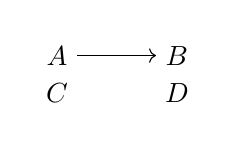
\begin{tikzpicture}
\matrix (m) [matrix of math nodes, column sep=1cm] { A & B \\ C & D \\ };
\draw[->] (m-1-1) -- (m-1-2);
\end{tikzpicture} \]

Dollars matrix.
$$ \begin{tikzpicture}
\matrix (m) [matrix of math nodes, column sep=1cm] { A & B \\ };
\draw[->] (m-1-1) -- (m-1-2);
\end{tikzpicture} $$

Bracket graphics.
\[ 
\includegraphics[alt={bracket graphics},width=2cm]{test-picture.png} \]

Dollars graphics.
$$ 
\includegraphics[alt={dollars graphics},width=2cm]{test-picture.png} $$

Displaymath tikzpicture.
\begin{displaymath}
\begin{tikzpicture}\draw (0,0) -- (2,1);\end{tikzpicture}
\end{displaymath}

Displaymath graphics.
\begin{displaymath}

\includegraphics[alt={displaymath graphics},width=2cm]{test-picture.png}
\end{displaymath}

Equation tikzpicture.
\begin{equation}
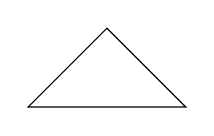
\begin{tikzpicture}\draw (0,0) -- (2,0) -- (1,1) -- cycle;\end{tikzpicture}
\label{eq:triangle}
\end{equation}

Equation star graphics.
\begin{equation*}

\includegraphics[alt={equation star graphics},width=2cm]{test-picture.png}
\end{equation*}

Equation star tikzcd.
\begin{equation*}
\begin{tikzcd} A \arrow[r] \arrow[d] & B \arrow[d] \\ C \arrow[r] & D \end{tikzcd}
\end{equation*}

Bracket picture environment.
\[ \begin{picture}(40,20)\put(0,0){\line(1,0){40}}\put(0,0){\line(2,1){40}}\end{picture} \]

Reference to the triangle: \ref{eq:triangle}.

\begin{theorem}
Theorem tikzpicture.
\[ 
\begin{tikzpicture}\draw (0,0) rectangle (1,1);\end{tikzpicture} \]
\end{theorem}

\begin{proof}
Proof tikzpicture.
\[ \begin{tikzpicture}\draw (0,0) -- (1,0);\end{tikzpicture} \qedhere \]
\end{proof}

Ordinary display.
\[ y = 1 \]

Ordinary dollars.
$$ a + b $$
\end{document}
